\chapter{Analysis}
\label{ch:analysis}
\section{Data Collection}
\subsection{Benchmark Targets} %what are we benchmarking on
Three SoCs have been created using the core designs in \ref{ch:hw_design}, two of which are homogeneous and a single heterogeneous design.

\begin{description}
    \item[B1] 1 big core - homogeneous
    \item[S2] 2 small cores - homogeneous
    \item[B1S1] 1 big core, 1 small core - heterogeneous
\end{description}

These designs have been chosen to give a spread of performance and area, comparing heterogeneous against homogeneous designs that will perform similarly to it. A 4th SoC of two big cores ('B2') has not been implemented, but would also be useful in comparisons between homogeneous and heterogeneous designs. This was not possible due to the limitations of the FPGA - a B2 SoC took up 65576 LUTs, while the available LUTs on the FPGA is only 63400.

\begin{figure}[h!]
    \centering
    \includegraphics*[width=\textwidth]{img/B2_lut_overuse.png}
    \caption{LUT overuse by B2 SoC}
    \label{fig:B2_lut_overuse}
\end{figure}

\subsection{Resource Usage} %todo finish this
\subsubsection{B1}
\begin{center}
\begin{tabular}{c c c c}
    Resource & Utilisation & Available & Utilisation \% \\
    \hline
    LUT	& 40991 & 63400 & 64.65458 \\
    \hline
    LUTRAM & 4027 & 19000 & 21.194736 \\
    \hline
    FF & 30567 & 126800 & 24.106466 \\
    \hline
    BRAM & 16 & 135 & 11.851851 \\
    \hline
    DSP & 4 & 240 & 1.6666667 \\
    \hline
\end{tabular}
\end{center}

\subsubsection{S2}
\begin{center}
\begin{tabular}{c c c c}
    Resource & Utilisation & Available & Utilisation \% \\
    \hline
    LUT	& 46201	& 63400	& 72.87224 \\
    \hline
    LUTRAM	& 4436 & 19000	& 23.347368 \\
    \hline
    FF & 31355 & 126800 & 24.727919 \\
    \hline
    BRAM & 9 & 135 & 6.666667 \\
    \hline
    DSP & 0 & 240 & 0.0 \\
    \hline
\end{tabular}
\end{center}

\subsubsection{B1S1}
\begin{center}
\begin{tabular}{c c c c}
    Resource & Utilisation & Available & Utilisation \% \\
    \hline
    LUT & 52423 & 63400 & 82.68612 \\
    \hline
    LUTRAM & 4540 & 19000 & 23.894735 \\
    \hline
    FF & 36720 & 126800 & 28.958992 \\
    \hline
    BRAM & 19 & 135 & 14.074074 \\
    \hline
    DSP & 4 & 240 & 1.6666667 \\
    \hline
\end{tabular}
\end{center}

\subsubsection{Graphical Comparison}
\begin{figure}[h!]
    \centering
    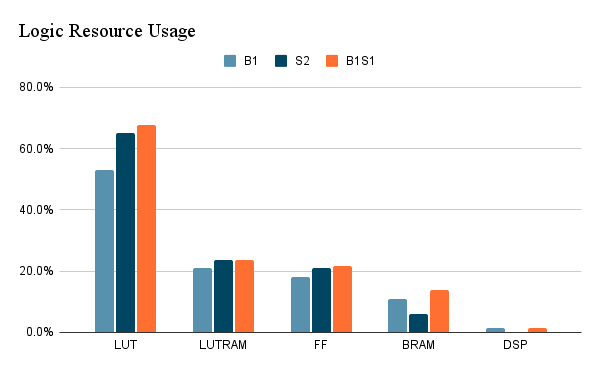
\includegraphics[width=\textwidth]{img/Logic Resource Usage.png}
    \caption{Resource comparison between SoCs}
    \label{fig:resource_soc_comp}
\end{figure}

\subsection{Estimated Power Usage}
\begin{center}
\begin{tabular}{c c c c c c}
    SoC & Total Power (W) & Clock (W) & Signal (W) & Logic (W) & BRAM (W) \\
    \hline
    B1 & 1.225 & 0.060 & 0.054 & 0.037 & 0.028 \\
    \hline
    S2 & 1.250 & 0.067 & 0.072 & 0.055 & 0.013 \\
    \hline
    B1S1 & 1.300 & 0.069 & 0.090 & 0.061 & 0.034 \\
    \hline
\end{tabular}
\end{center}

\subsection{Performance and Temperature}
Performance data was collected using multiple runs of each benchmark. Each benchmark-SoC combination was loaded to the FPGA and run five times, with the average cycle counts being recorded for each. The benchmarks can be varied in size, and we ran several versions to identify how a longer benchmark with larger amounts of data affected the performance of each SoC.

Raw results of the benchmarks can be seen in \ref{ch:appendix}.

\subsubsection{Addition Graph}

\begin{figure}[H]
    \centering
    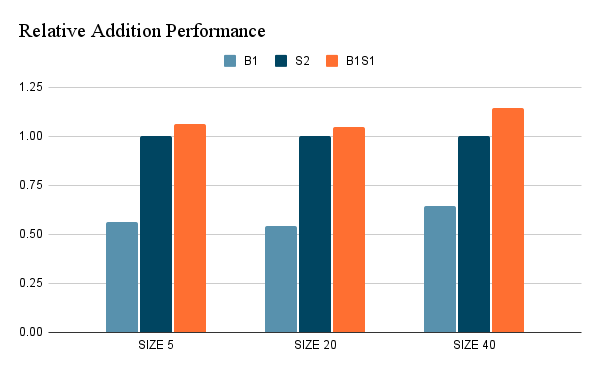
\includegraphics[width=0.7\textwidth]{img/Relative Addition Performance.png}
    \caption{Relative Addition Performance of SoCs}
    \label{fig:add_relative_graph}
\end{figure}

\subsubsection{Multiplication Graph}

\begin{figure}[H]
    \centering
    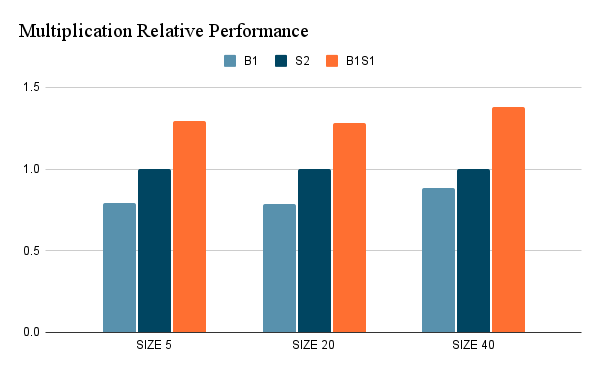
\includegraphics[width=0.7\textwidth]{img/Multiplication Relative Performance.png}
    \caption{Relative Multiplication Performance of SoCs}
    \label{fig:mul_relative_graph}
\end{figure}

\subsubsection{IO Graph}

\begin{figure}[H]
    \centering
    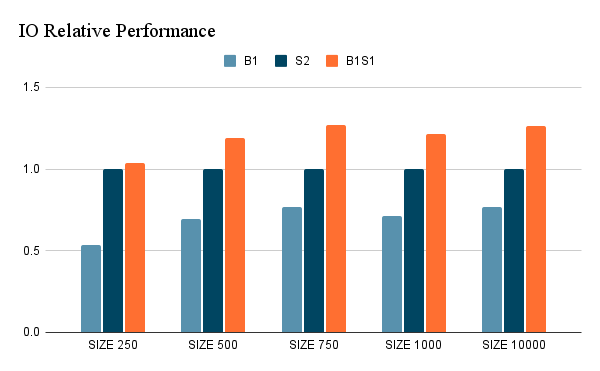
\includegraphics[width=0.7\textwidth]{img/IO Relative Performance.png}
    \caption{Relative IO Performance of SoCs}
    \label{fig:IO_relative_graph}
\end{figure}

\subsubsection{Mixed Graph}

\begin{figure}[H]
    \centering
    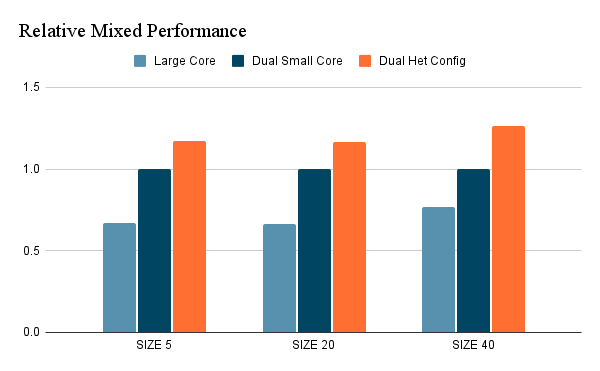
\includegraphics[width=0.7\textwidth]{img/Relative Mixed Performance.png}
    \caption{Relative Mixed Performance of SoCs}
    \label{fig:mix_relative_graph}
\end{figure}

\subsubsection{Temperature}
Temperature measurement has been done as a substitute power measurement. While voltage to the FPGA chip can be measured on the board, there are no current measurements and we cannot find the actual power consumed during the benchmarks. It would be possible to measure current draw through the USB port that powers the board, but this would require the use of a USB cable with inbuilt power measurement and display. The power draw through the cable would also include static components, such as the board RAM, LEDs, etc, and make it difficult to accurately measure the correct power draw by each SoC. This makes this method of measuring power unsuitable for our project. Instead, temperature will be used to order the SoCs in terms of power draw. 

To generate the temperature data we ran the mixed benchmark on each SoC in a single room over a few hours. This was to attempt to keep the ambient room temperature approximately the same for all runs, which would affect the peak temperature measurement. The mixed benchmark was compiled with size 40 and 100000 iterations instead of the normal 100, ensuring the time taken to complete the benchmark was adequately long for the FPGA to reach a stable temperature. The methodology for finding peak temperature is given below:

\begin{enumerate}
    \item SoC bitstream is written to the FPGA
    \item 10-minute waiting period for FPGA to reach stable base temperature
    \item Benchmark is transferred to the SoC via serial debugger
    \item Benchmark is run for 10 minutes
    \item Peak temperature over time the benchmark is running is recorded
\end{enumerate}

We also changed the SoCs being tested in this benchmark from the one specified previously, as well as how the benchmark is being run on the SoC. An S1 SoC has been included, with the S2 SoC removed, and the benchmark has been run on the S core in B1S1 individually, showing a situation where the B core is idle and only the S core is necessary for computation. This has been done to enable 'power' measurements for situations where the heterogeneous SoC is most effective.

\begin{figure}[H]
    \centering
    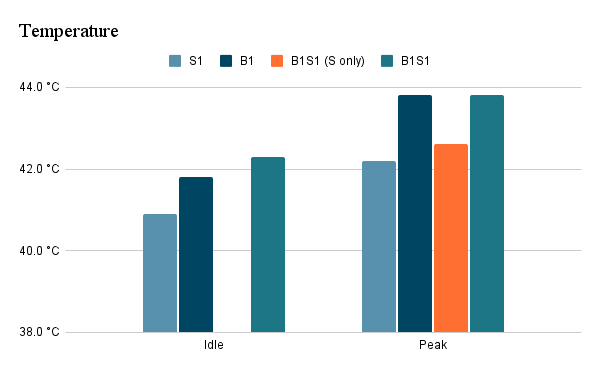
\includegraphics[width=0.6\textwidth]{img/Temperature.png}
    \caption{Temperature measurements at idle and peak}
    \label{fig:soc_temps}
\end{figure}

\section{Performance/Power Analysis}
\subsection{Addition Benchmark}
\begin{center}
\begin{tabular}{c c c c}
    SoC & Size 5 & Size 20 & Size 40 \\
    \hline
    B1 & 0.4612 & 0.4449 & 0.5265 \\
    \hline
    S2 & 0.8000 & 0.8000 & 0.8000 \\
    \hline
    B1S1 & 0.8192 & 0.8038 & 0.8808\\
    \hline
\end{tabular}
\end{center}
In the addition benchmark, the B1S1 achieves the best performance/power ratio for all sizes. S2 and B1S1 are similar in ratio for sizes 5 and 20, but the differences increases significantly as the size increases to 40 and the increased cache in the B core has a greater effect. The general trend is increasing in size and amount of cores increases performance faster than power draw increases.

\subsection{Multiplication Benchmark}
\begin{center}
\begin{tabular}{c c c c}
    SoC & Size 5 & Size 20 & Size 40 \\
    \hline
    B1 & 0.6465 & 0.6396 & 0.7192 \\
    \hline
    S2 & 0.8000 & 0.8000 & 0.8000 \\
    \hline
    B1S1 & 0.9938 & 0.9873 & 1.0623\\
    \hline
\end{tabular}
\end{center}
B1S1 again achieves the best performance/power ratio for all sizes, with the relative performance of the B cores increasing as the size increases. The general trend again is that increasing the size and amount of cores increases performance more than power.

\subsection{Mixed Benchmark}
\begin{center}
\begin{tabular}{c c c c}
    SoC & Size 5 & Size 20 & Size 40 \\
    \hline
    B1 & 0.5465 & 0.5424 & 0.6253 \\
    \hline
    S2 & 0.8000 & 0.8000 & 0.8000 \\
    \hline
    B1S1 & 0.8996 & 0.8958 & 0.9738\\
    \hline
\end{tabular}
\end{center}
For the mixed benchmark, the SoC with the best performance/power ratio is B1S1 for all sizes. The general trend is increasing the size and amount of cores leads to a larger increase in performance than estimated power consumption.

\section{Conclusions}
Taken in isolation, the data appears to show that heterogeneous designs show massive benefits over homogeneous designs. Compared to the B1 SoC, the B1S1 achieves performance increases of up to 88\%, for only 6\% increase in power consumption and a 15-30\% resource utilisation increase depending on the exact resource being compared. The B1S1 also produces up to 38\% performance increase compared to the S2 SoC, with just 4\% increase in power and ~5\% resource utilisation increase. 

However, we believe these results do not show heterogeneous designs being superior in FPGAs, but that larger designs that use up more of the FPGA chip provide better performance/power and performance/area ratios. This is due to a large amount of the area utilised by the FPGA being from the rest of the SoC (from IO hardware, memory, etc) that is static between core designs, resulting in a large amount of static power draw between SoCs. The measurement of performance/power is also flawed in that the power is based on estimations by software. While this can provide an estimated ordering of power consumption - we can be relatively sure that a design with greater predicted power than another will actually consume more - this value is unsuitable for use in supporting claims that an SoC is purely better than another in terms of performance/power ratio.

\begin{figure}[h!]
    \centering
    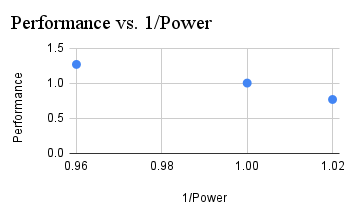
\includegraphics[width=0.5\textwidth]{img/Performance vs. 1_Power.png}
    \caption{Performance vs. 1/Power in SoCs}
    \label{fig:perf_v_power}
\end{figure}

Figure \ref{fig:perf_v_power} shows that while there are huge differences in performance between the SoCs, the inverse changes to power result in each SoC being a pareto point.

The data in figure \ref{fig:soc_temps} shows some evidence that heterogeneous designs in FPGAs may provide benefits when only the S core is in use. There is a measurable, though small, decrease in temperature when using only the S core in the B1S1 SoC. The temperature is very close to the S1 SoC, implying the power draw by the idle B core is very small and in situations where only the S core is necessary, the B1S1 SoC could have a tangible decrease in power draw. Some flaws in the testing methodology could mean this result is not accurate. For instance, the benchmark fully leverages any CPU it is running on and would run faster on a faster core. This means the B core is actually doing more work than the S core in the same time-period and does not have the same workload over the benchmark duration. Decreasing the amount of work done by the B core to the same amount as the S core could see the temperature reduce to the same as if the S core was in use, meaning the S core has no benefit in the system. Another issue with this conclusion is the use of temperature to estimate power draw. This is undoubtedly inaccurate, and it would be hard to justify conclusions based on a temperature difference of less than 2$^{\circ}$C.